\documentclass[conference, 10ppt]{IEEEtran}
\usepackage{amsmath,amssymb,amsfonts}
%\usepackage{algorithmic}
\usepackage{graphicx}
\usepackage{textcomp}
\usepackage{xcolor}
\usepackage{comment}
%
%\usepackage{slashbox}
\usepackage{url}
\usepackage{cite}
\usepackage{amsmath,amssymb,amsfonts}
\usepackage{graphicx}
\usepackage{textcomp}
\usepackage{xcolor}
\usepackage{algorithm,algpseudocode}
\algrenewcommand\algorithmicindent{0.9em}%
\usepackage{soul}
\usepackage{xspace}
\usepackage{subfigure}
\usepackage[group-separator={,}, group-minimum-digits=4]{siunitx}
\usepackage{makecell}
\usepackage{multirow}
\usepackage{xcolor,colortbl}

%
\def\BibTeX{{\rm B\kern-.05em{\sc i\kern-.025em b}\kern-.08em
    T\kern-.1667em\lower.7ex\hbox{E}\kern-.125emX}}
 
\begin{document}
%
\newcommand{\todo}[1]{\color{red}\textbf{\hl{#1}}\color{black}\xspace}
%\newcommand{\todo}[1]{}
\newcommand{\rom}[1]{\expandafter{\romannumeral #1\relax}}
%
\title{Performance Model of Iterated SpMV for Distributed System.}

\author{\IEEEauthorblockN{Md Maruf Hossain}
\IEEEauthorblockA{Dept. Computer Science \\
\textit{University of North Carolina at Charlotte}\\
Charlotte, USA \\
mhossa10@uncc.edu}
\and
\IEEEauthorblockN{Erik Saule}
\IEEEauthorblockA{Dept. Computer Science \\
\textit{University of North Carolina at Charlotte}\\
Charlotte, USA \\
esaule@uncc.edu}
}
%
%%
%%
\maketitle
%%

\begin{abstract}
Many applications rely on basic sparse linear algebra operations from numerical solvers to graph analysis 
algorithms. Yet, the performance of these operations is still reasonably unknown. Users and practitioners 
rely on the rule of thumb understanding of what typically works best for some application domain.
\\ 
This paper aims at providing an overall framework for the distributed system to think about the performance 
of sparse applications. We use the sparse matrix-vector(SpMV) multiplication as the representative of the 
experiments. We model the performance of multiple SpMV implementations on distributed systems. 
 We model the performance of different modes of execution of SpMV using linear and polynomial regression models for a distributed system. 
 The models enable us to predict how to partition and represent the sparse matrix to optimize the performance of iterated SpMV on a cluster with 225 cores.
\end{abstract}
%
%%
%%

\begin{IEEEkeywords}
SpMV, MPI, Graph Partitioning
\end{IEEEkeywords}

\section{Introduction}
%%%%%%%%% Why %%%%%%%%%
Sparse matrix-vector multiplication(\textit{SpMV}) is one of the
fundamental operations in sparse linear algebra. It is critical to
solving linear systems and is widely used in engineering and scientific
applications~\cite{gleich2015pagerank, saad2003iterative, dytrych2016efficacy}. 
Distributed memory systems have entered a new age with
the popularization of departmental clusters to support these
scientific and engineering applications.  Many different approaches
have been proposed to improve \textit{SpMV} performance on
clusters. But choosing the right approach still mostly relies on the rule
of thumbs. We posit that building models to predict the performance of
different configurations is the only way to make better-informed
decisions.

In this paper, we propose a linear and polynomial \textit{Support
  Vector Regression}(\textit{SVR})~\cite{awad2015support} model to predict and analyze the
run time of \textit{SpMV} on the distributed system for different ways
to execute the operation. Our system will analyze the predicted run
time and return the best possible algorithm for the system. The
performance of the \textit{SpMV} mainly depends on the size and
structure of the matrices and the architecture of the system. 

%%%%%%%%% How %%%%%%%%
To perform sparse matrix-vector multiplication(\textit{SpMV}) on
distributed systems, the most common mechanism is to partition the
matrix into multiple parts and perform \textit{SpMV} on each part
individually in the different processors. Good partitioning can ensure
better load balance and limits the volume of communication between the
underlying \textit{MPI process}. Many partitioning
algorithms have been proposed to ensure good load balance and to
minimize \textit{MPI communications}~\cite{deveci2015hypergraph, karypis1995multilevel,
  kaya2013analysis}.

%%%%%%%%% What %%%%%%%%
In this paper, we explore two partitioning modes (Uniform
2D-Partitioning and 1D Row Partitioning) and the performance of the
different \textit{SpMV} representation based on these partitioning
mechanisms on distributed systems. We develop a linear and a
polynomial support vector regression (\textit{SVR}) performance models
for SpMV operations on the distributed system for these different
techniques. The models are accurate enough to predict the best
configuration to execute SpMV given a matrix.


\section{\todo{SpMV on AVX-512 Architecture (Skylake)}}
SpMV on the distributed system initially can be divided into two parts, 
\begin{itemize}
\item MPI Communication: latency to share the vector and gather the results from the MPI process. 
\item Core SpMV Calculation: latency to calculate part of SpMV for a single MPI process.
\end{itemize}

\subsection{MPI communication}

\subsection{Core SpMV Calculation}
We can represent the basic SpMV by $y=y+Val*x$, which contains two floating point operation(multiply and addition). 
So, we can say we need to calculate NNZ(number of non zeros) times FMA(fused multiply addition) to perform SpMV.
In our experiment we divide the core SpMV calculation into two major parts,
\begin{itemize}
\item Run time for FMA: $L_{FMA}\times NNZ$, where $L_{FMA}$ is the latency of a single FMA and $NNZ$ is number of nonzeros.
\item Read-write latency: $L_{RW}$
\end{itemize} 

\subsubsection{Memory Access bandwidth}
\begin{figure}[hbt!]
	\centering
	\subfigure[Single Precision.]{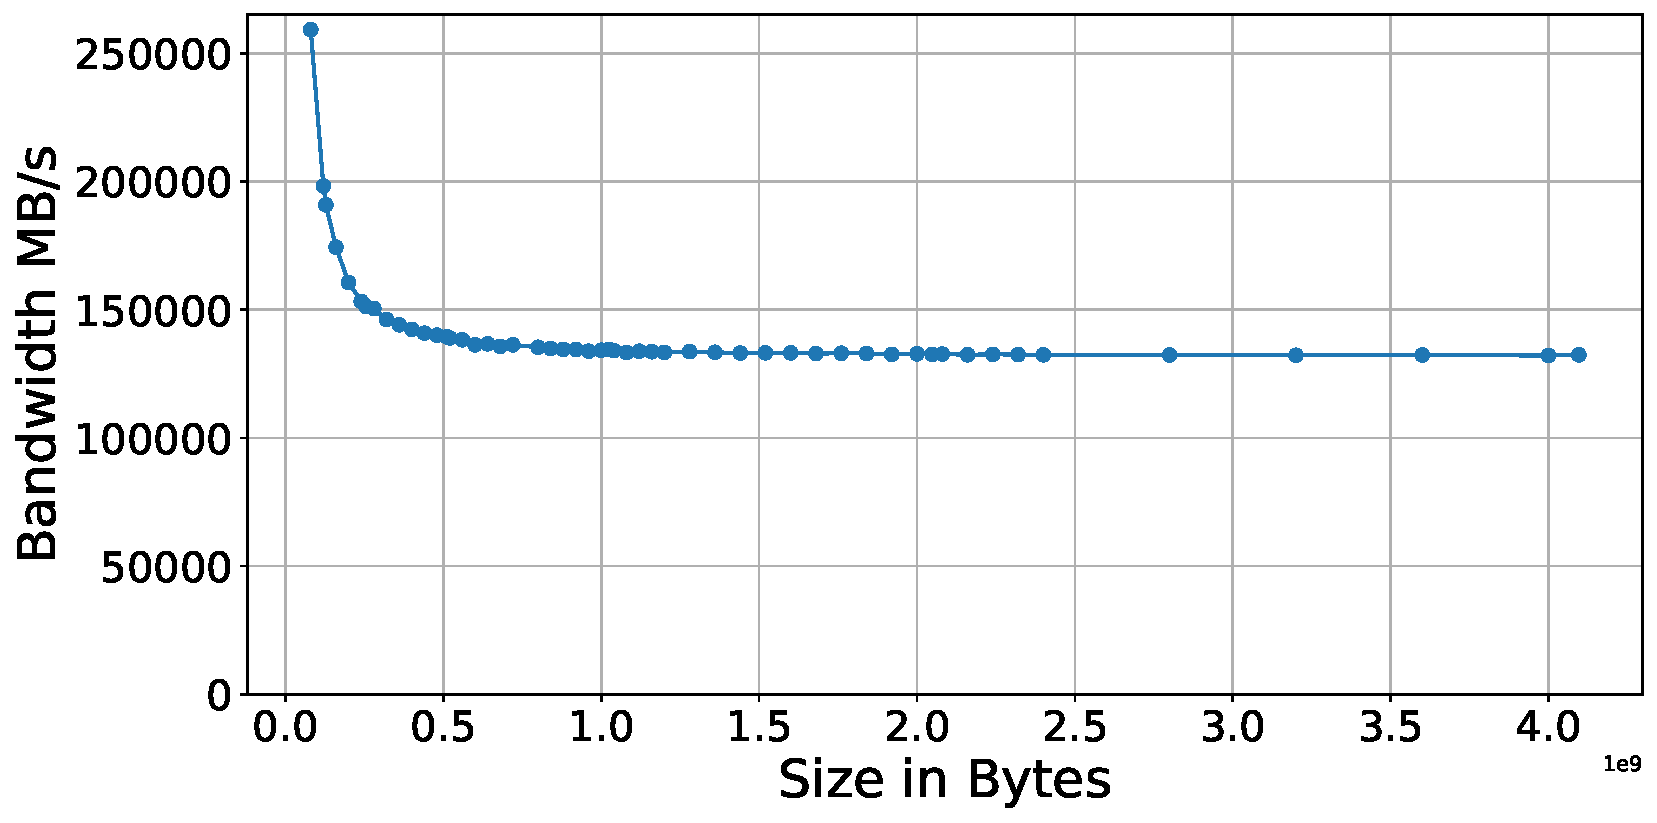
\includegraphics[width=0.48\linewidth]{figures/stream/skylake_mpi_copy_single_precision.pdf}		\label{fig:stream-single-copy}}
	\subfigure[Double Precision.]{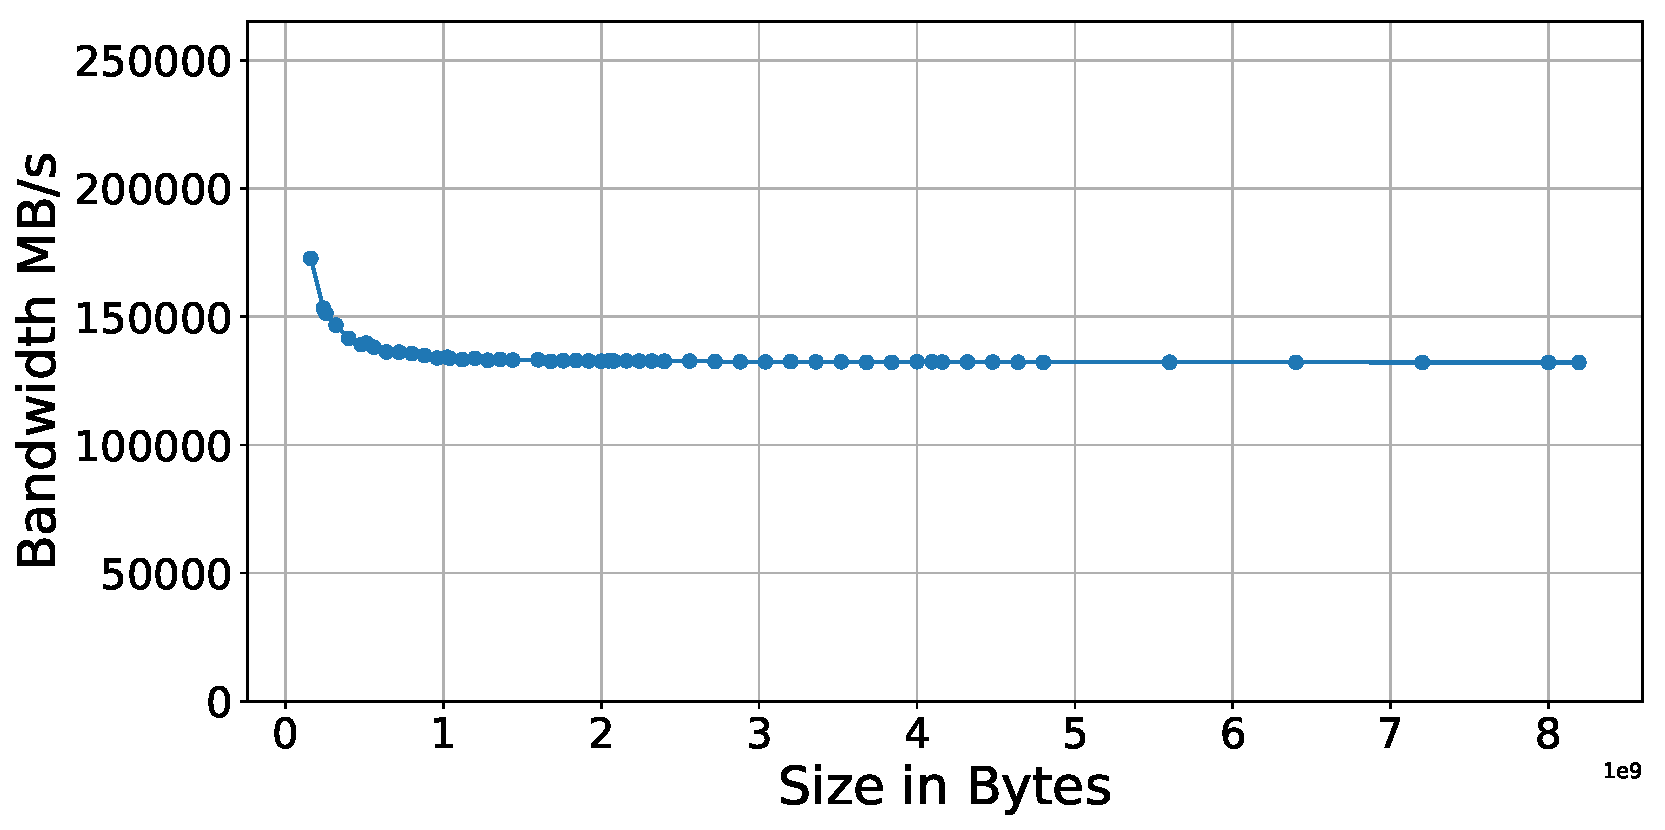
\includegraphics[width=0.48\linewidth]{figures/stream/skylake_mpi_copy_double_precision.pdf}		\label{fig:stream-double-copy}}
	\caption{Single and double precision memory access bandwidth on Skylake processor.}
	\label{fig:stream-copy-bandwidth}
\end{figure}
Figure~\ref{fig:stream-copy-bandwidth} shows, when the size of the data is more than 1GB the bandwidth shows the consistency 
with the size of the data(132 GB/s).


\subsubsection{Roofline Model for FMA}
The throughput of Skylake and Cascade Lake are same as 2 instructions per cycle and the latency of FMA is 4 cycles for both of them. So there is a potential of pipelinling($2\times 4 = 8$) to get the optimal results. Now, both of the architecture 
has 512-bit register that can give the ability of the vectorization. For 64-bits floating point operation it can give vector 
width 8 and for 32-bits it can give at max vector width 16. To find the peak performance of the FMA and to avoid the 
read-write latency we need to setup the benchmark that datasets can be contained in the register. Now, both of the 
architecture have 32 registers. We can populate the pipeline by using sufficient ampunt of work. By varying the 
number of fused-multiply-addition calculation, we can find out the performance limitation. From the informations of the 
processors, we can say that 4 cycles required for FMA and the throughput of the FMA is 2 instruction per cycle, that means 
we should at least use $4\times 2=8$ instruction at a time to populate the pipeline.

\begin{figure}[hbt!]
	\centering
	\subfigure[Vector Width: 4]{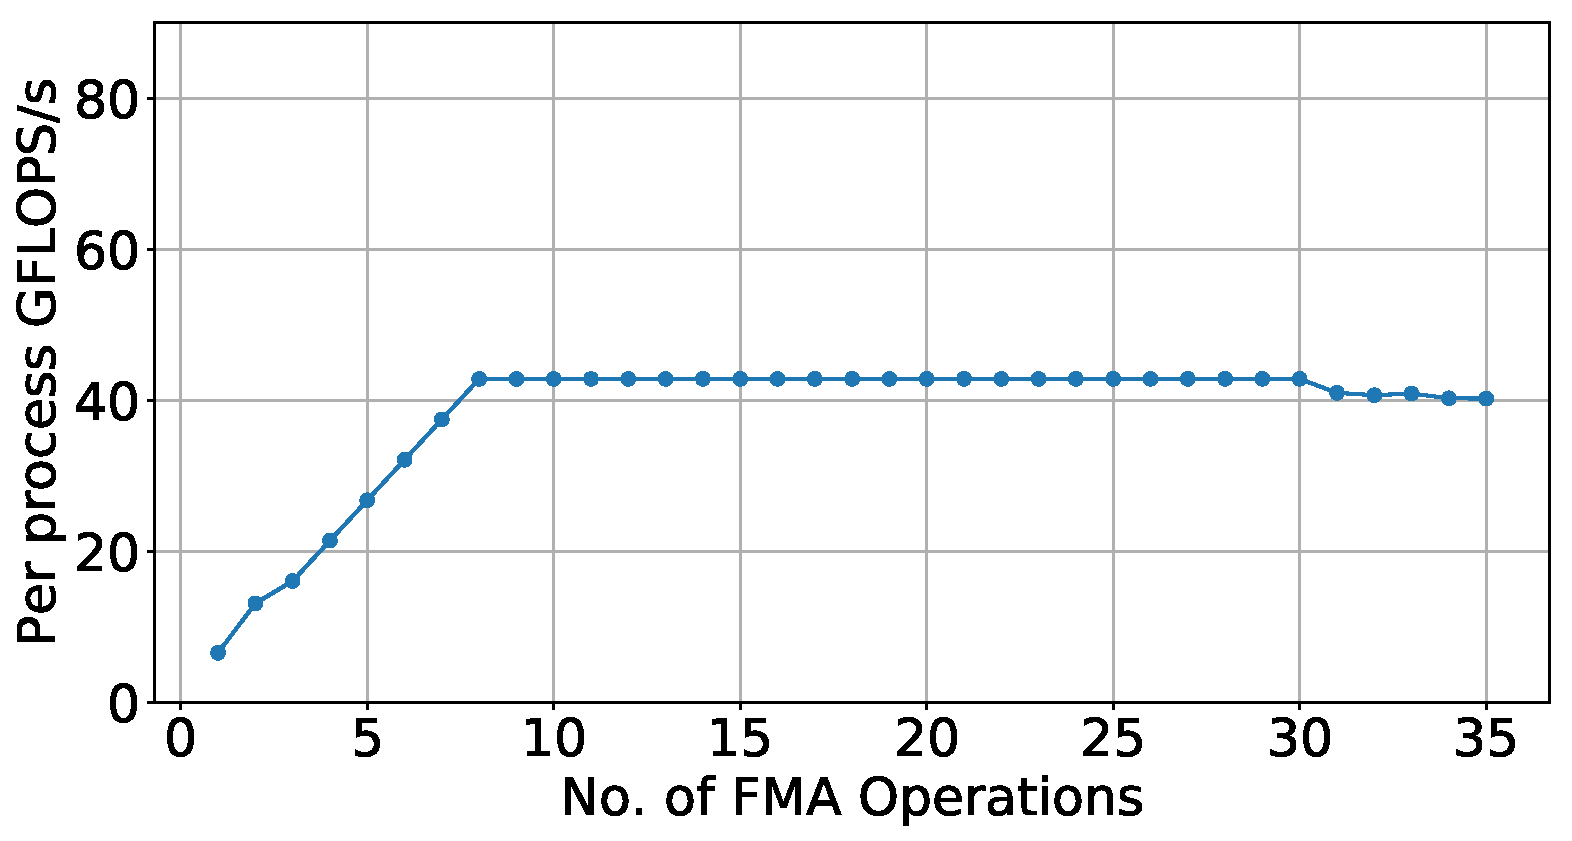
\includegraphics[width=0.48\linewidth]{figures/skylake_mpi_fma_roofline_model_for_vec_4.pdf}		\label{fig:mpi-skl-vec-4}}
	\subfigure[Vector Width: 8]{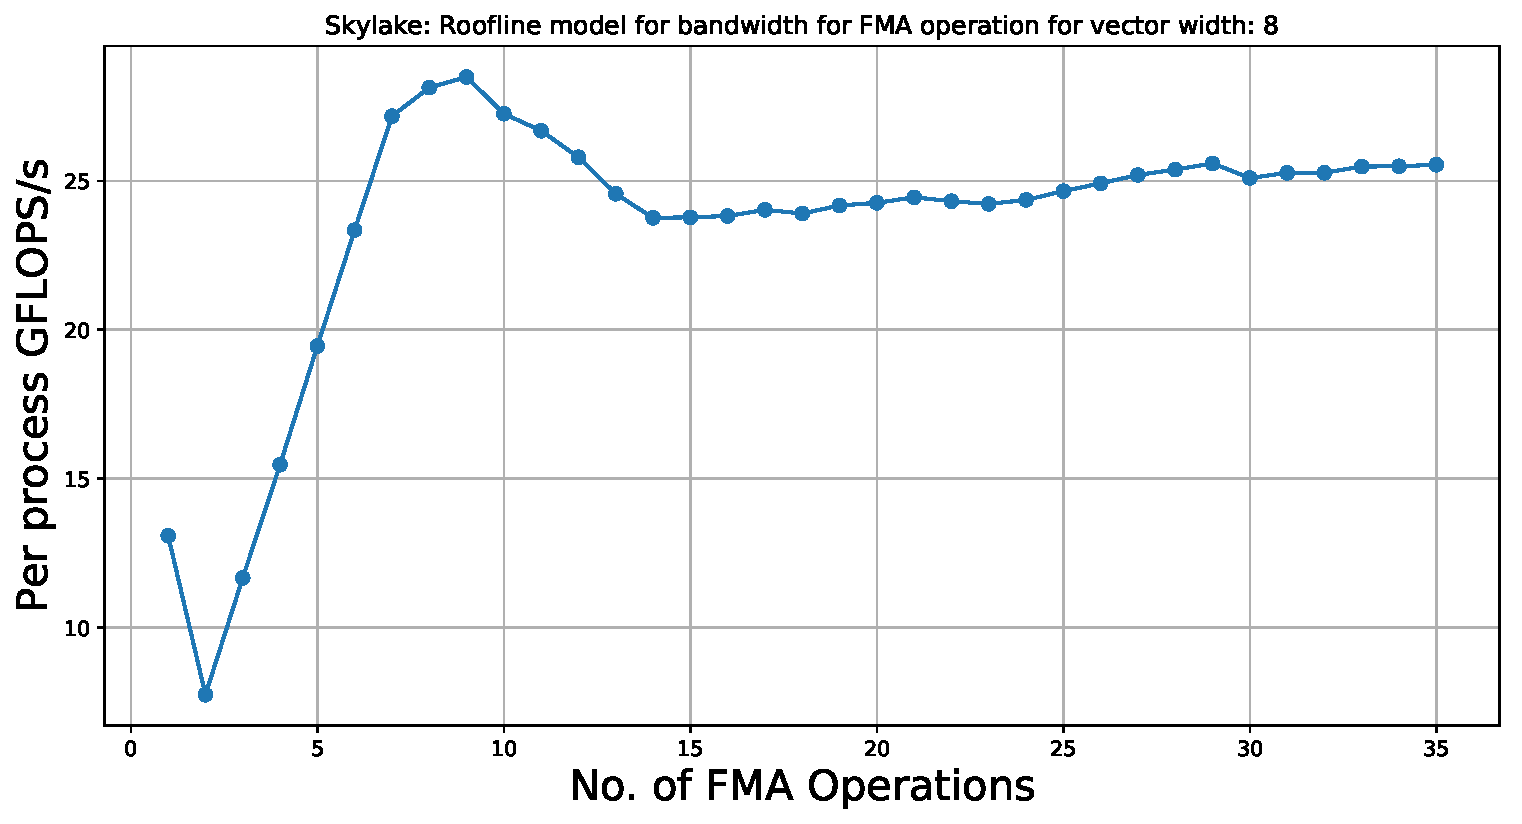
\includegraphics[width=0.48\linewidth]{figures/skylake_mpi_fma_roofline_model_for_vec_8.pdf}		\label{fig:mpi-skl-vec-8}}
	\caption{Skylake: (MPI)Roofline model for bandwidth for FMA operation}
	\label{fig:mpi-skl-roofline}
\end{figure}


\begin{figure}[hbt!]
	\centering
	\subfigure[Vector Width: 4]{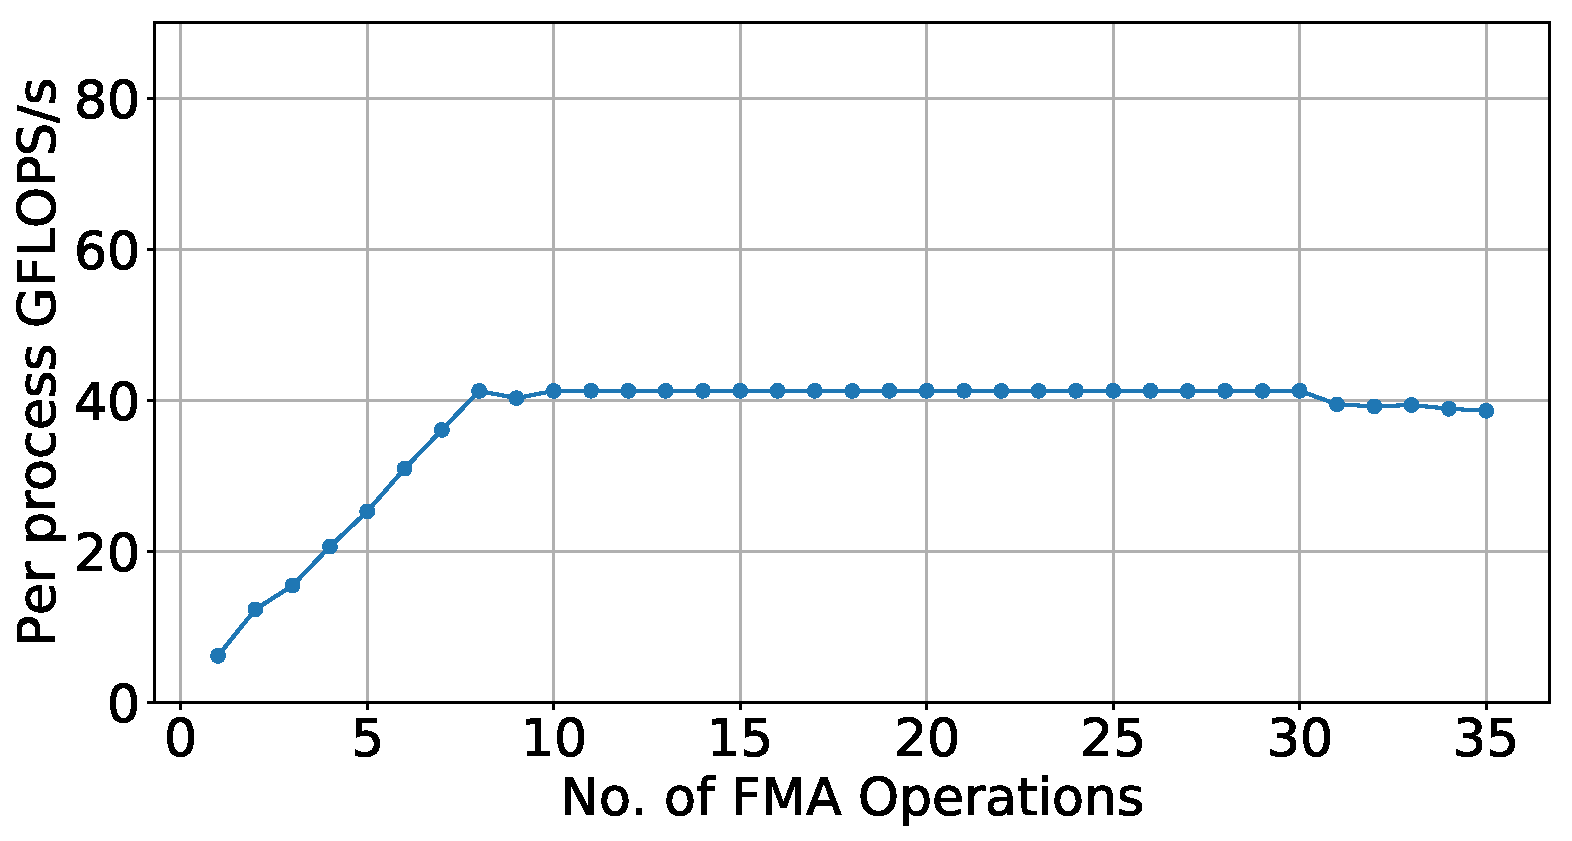
\includegraphics[width=0.48\linewidth]{figures/cascade_lake_mpi_fma_roofline_model_for_vec_4.pdf}		\label{fig:mpi-cas-vec-4}}
	\subfigure[Vector Width: 8]{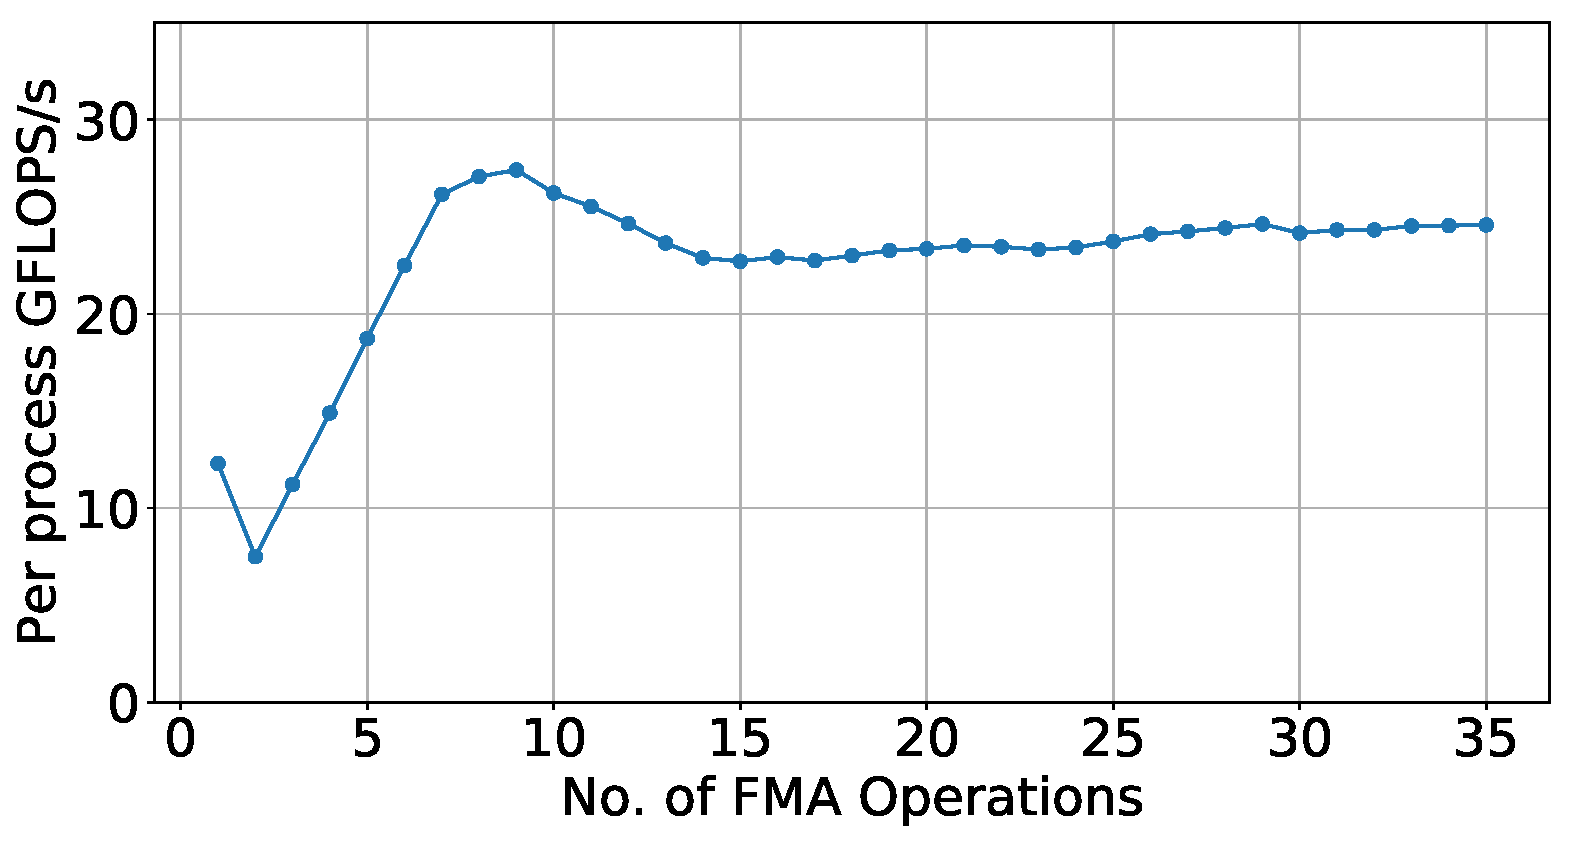
\includegraphics[width=0.48\linewidth]{figures/cascade_lake_mpi_fma_roofline_model_for_vec_8.pdf}		\label{fig:mpi-cas-vec-8}}
	\caption{Cascade Lake: (MPI)Roofline model for bandwidth for FMA operation}
	\label{fig:mpi-cas-roofline}
\end{figure}


\begin{figure}[hbt!]
	\centering
	\subfigure[Vector Width: 4]{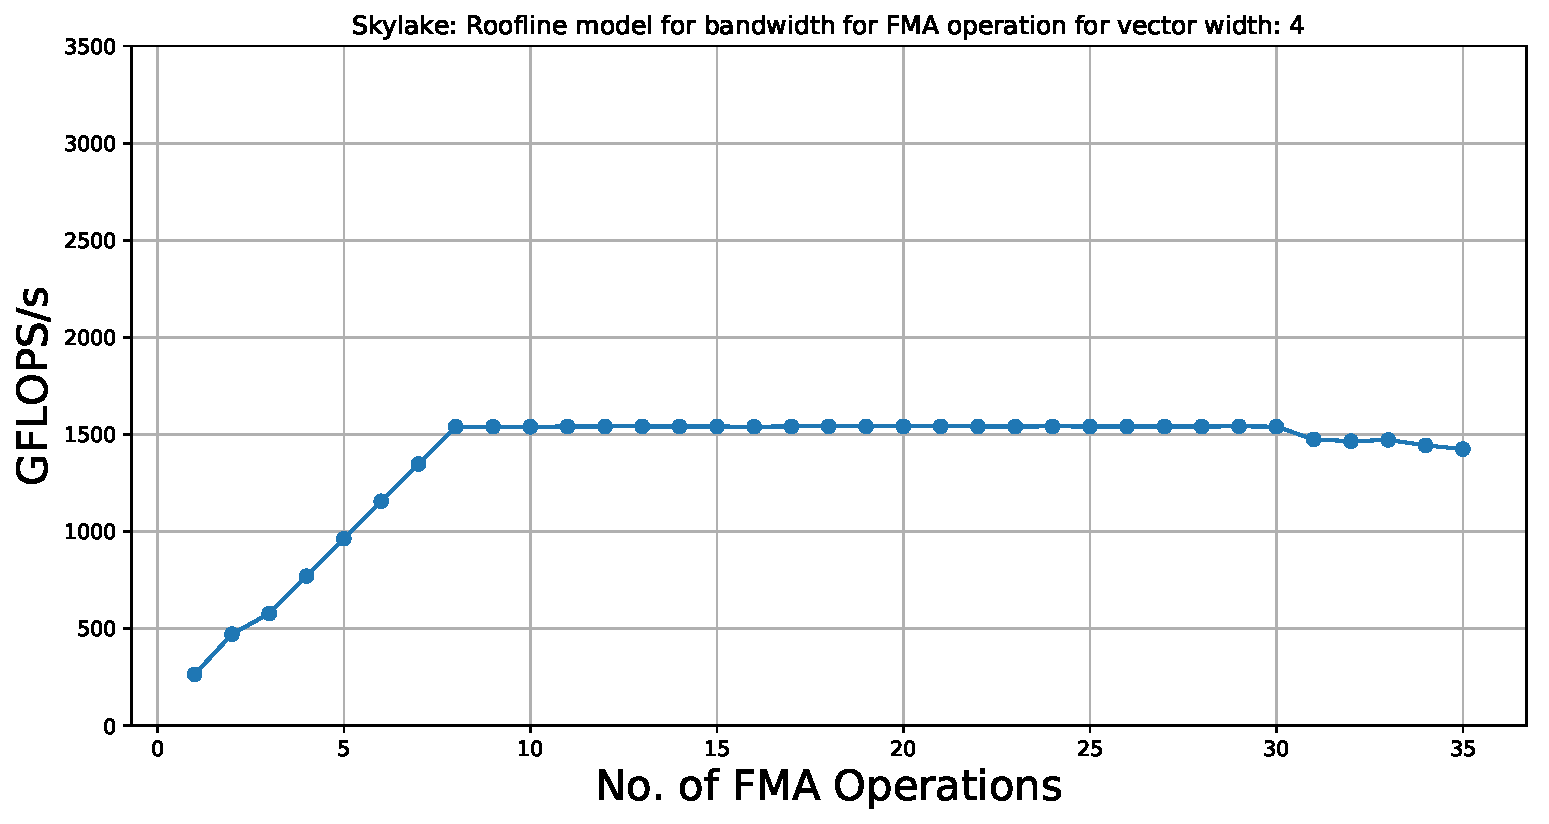
\includegraphics[width=0.48\linewidth]{figures/skylake_omp_fma_roofline_model_for_vec_4.pdf}		\label{fig:omp-skl-vec-4}}
	\subfigure[Vector Width: 8]{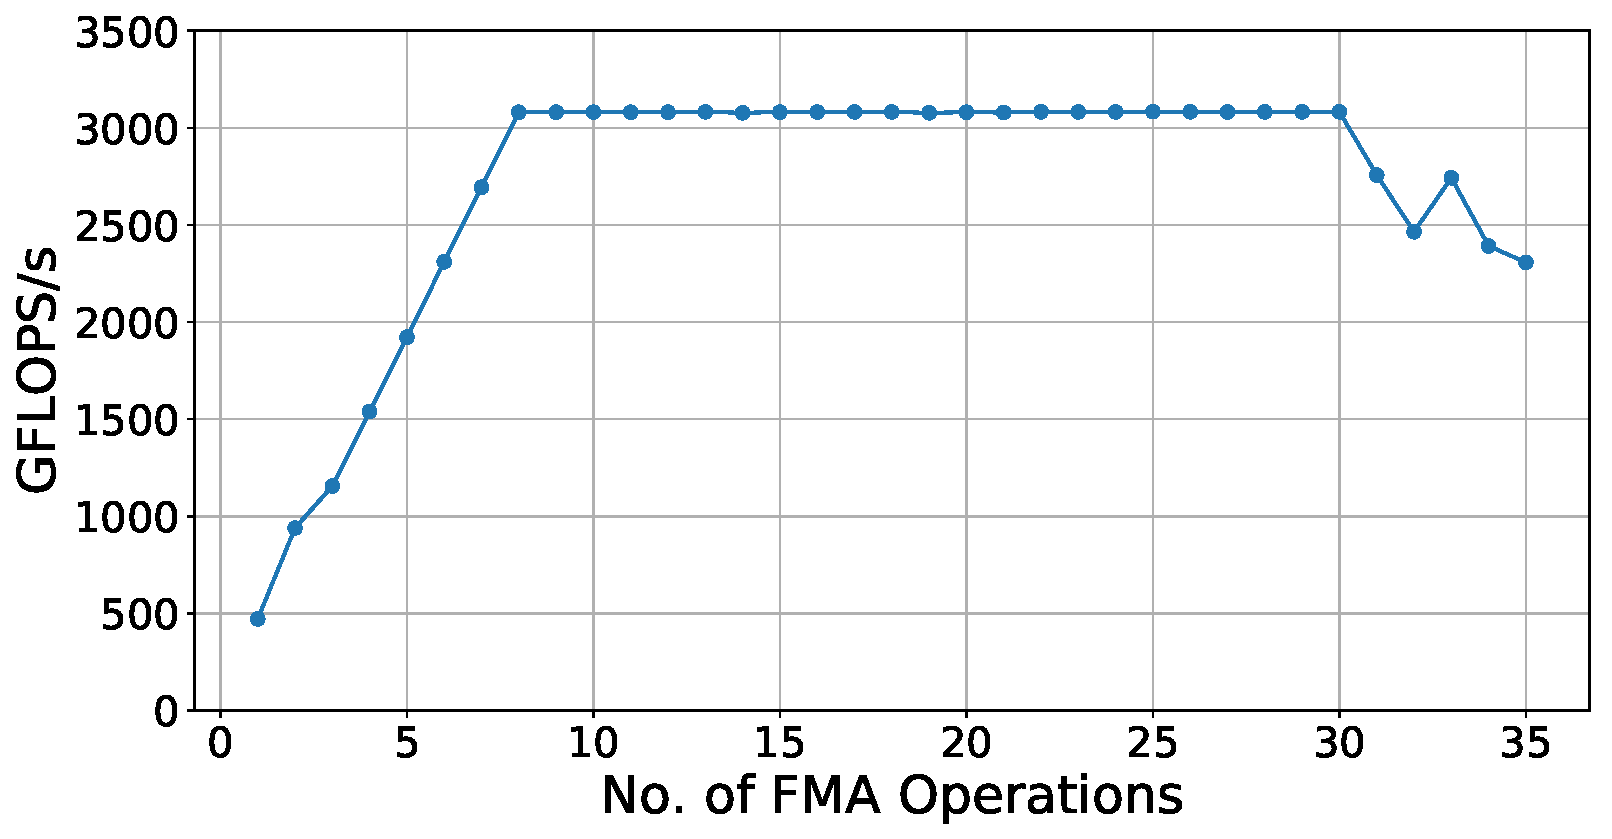
\includegraphics[width=0.48\linewidth]{figures/skylake_omp_fma_roofline_model_for_vec_8.pdf}		\label{fig:omp-skl-vec-8}}
	\caption{Skylake: (Shared memory parallel)Roofline model for bandwidth for FMA operation}
	\label{fig:omp-skl-roofline}
\end{figure}


\begin{figure}[hbt!]
	\centering
	\subfigure[Vector Width: 4]{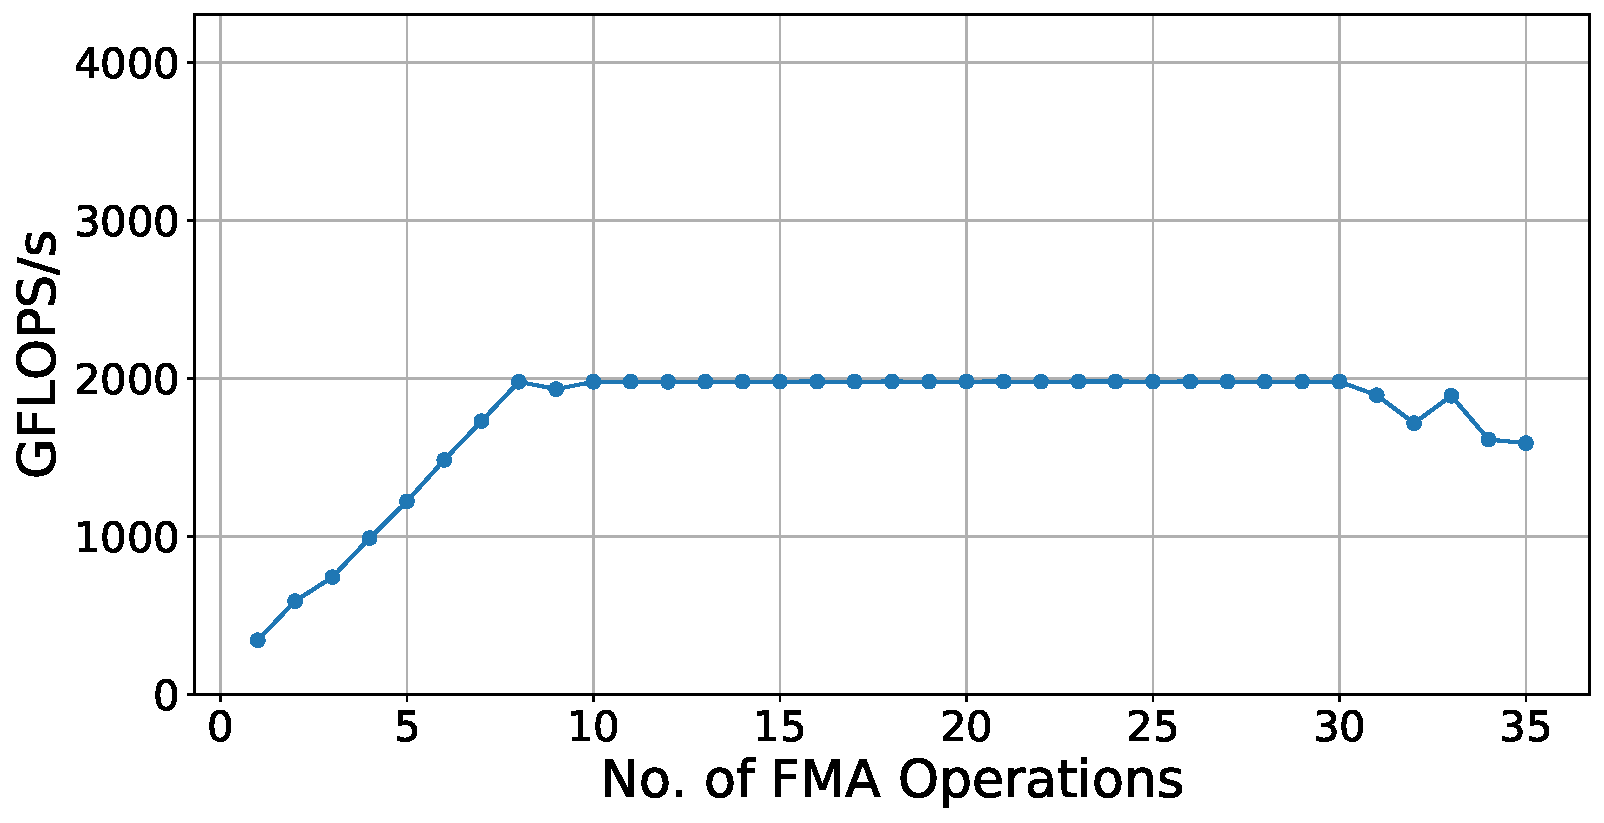
\includegraphics[width=0.48\linewidth]{figures/cascade_lake_omp_fma_roofline_model_for_vec_4.pdf}		\label{fig:omp-cas-vec-4}}
	\subfigure[Vector Width: 8]{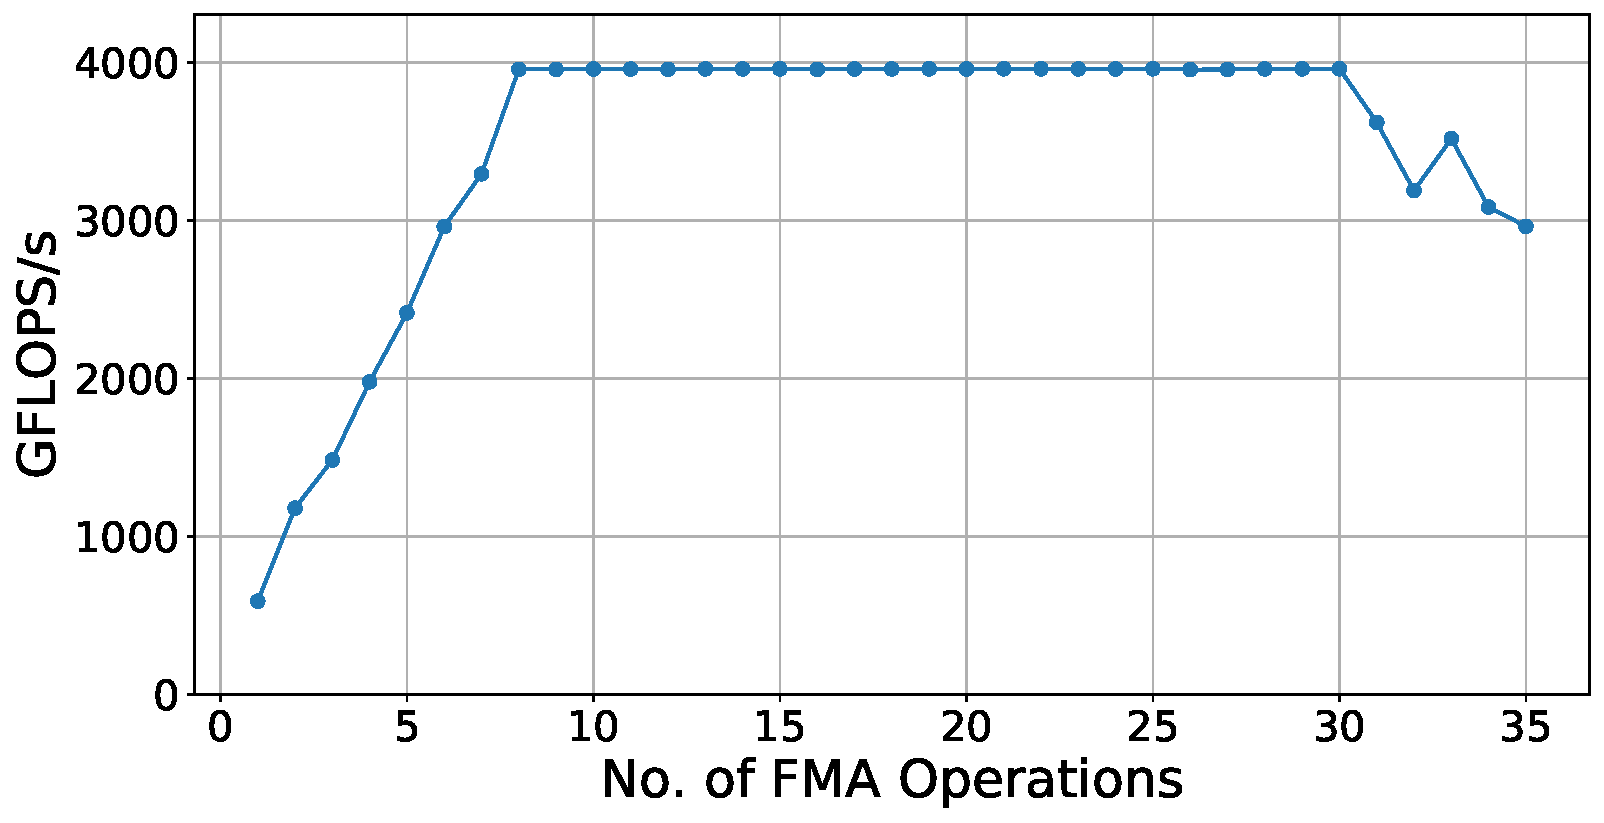
\includegraphics[width=0.48\linewidth]{figures/cascade_lake_omp_fma_roofline_model_for_vec_8.pdf}		\label{fig:omp-cas-vec-8}}
	\caption{Cascade lake: (Shared memory parallel)Roofline model for bandwidth for FMA operation}
	\label{fig:omp-cas-roofline}
\end{figure}

We can estimate the theoritical peak performance a single FMA by the following equation,
\begin{eqnarray}
P\ =\ Base\_Clock\_Frequency\times Vector\_Width\times \frac{FLOPs}{Instruction}.
\end{eqnarray}


\bibliographystyle{unsrt}
\bibliography{spmv}
\end{document}